\documentclass{beamer}

\usepackage{chemfig}
\usepackage[siunitx]{circuitikz}
\usepackage{dsfont}
\usepackage{fancyvrb}
\usepackage{pgfplots}
\usepackage{tcolorbox}
\usepackage{tikz}

\tcbuselibrary{listings}

\usetikzlibrary{arrows, cd, trees}
\tikzset{
    state/.style={
		circle,
        draw=black, thick,
        minimum width=.75cm,
        minimum height=.75cm,
        inner sep=2pt,
        text centered,
     },
}
\pgfplotsset{width=10cm,height=7.5cm,compat=1.3,tick label style={font=\scriptsize}}

\newcommand{\C}{\mathds{C}}
\newcommand{\D}{\mathds{D}}

%%--------------------------------------
%\usecolortheme{uwl}
\title{A Brief Introduction to \LaTeX}
\subtitle{Some Useful Packages for Everyday Things}
\author{Robert Allen}
\institute{Professor of Mathematics\\University of Wisconsin-La Crosse}
\date{\today}
\beamertemplatenavigationsymbolsempty

\begin{document}

\maketitle

\begin{frame}[t]
\frametitle{The Many Joys of \LaTeX}

\TeX\ was a typesetting system that was developed to typeset mathematics.  

\bigskip

\pause 
Seeing the usefullness of the system, people expanded upon it by adding functionality, thus developing what is now known as \LaTeX.

\bigskip

\pause
\LaTeX\ can be used to develop many useful documents that contain mathematics and complicated diagrams:
\begin{itemize}
	\item Papers and reports
	\item Presentation slides
	\item Large-scale posters
	\item Sheet music
	\item and the list goes on, and on, and on $\cdots$
\end{itemize}
	
\end{frame}

\begin{frame}[fragile,t]
\frametitle{How Do We Get Started?}

The essential elements of any \LaTeX\ document is the following template

\medskip

\begin{tcolorbox}[colback=red!5!white,colframe=red!75!black]
\begin{Verbatim}
\documentclass{article}

% load packages here

\begin{document}
    Hello, World!
\end{document}
\end{Verbatim}
\end{tcolorbox}

\medskip

\pause
The document class \textbf{article} is the beginning of most documents that resemble a paper.  If you wanted to create a slide presentation or poster, we would use a different document class.

\end{frame}

\begin{frame}[fragile,t]
\frametitle{Typesetting Mathematics}

Math mode is tagged by either using single \$ for inline text, or double \$ for full display.

\medskip

\begin{tcblisting}{colback=red!5!white,colframe=red!75!black}
If $\psi$ is the constant function 1, then $W_{\psi,\varphi} = C_\varphi$, $\|\psi\|_{\mathcal{B}} = 1$,$\sigma_{\psi,\varphi} = 0$, and $$\tau_{\psi,\varphi} = \sup_{z\in\D} \frac{1-|z|^2}{1-|\varphi(z)|^2}|\varphi'(z)|.$$
\end{tcblisting}
\end{frame}

\begin{frame}[fragile]	
\frametitle{Typesetting Mathematics}

\begin{tcblisting}{colback=red!5!white,colframe=red!75!black}
If $\psi$ is the constant function 1, then $W_{\psi,\varphi} = C_\varphi$, $\|\psi\|_{\mathcal{B}} = 1$,$\sigma_{\psi,\varphi} = 0$, and \begin{equation}\tau_{\psi,\varphi} = C_\varphi \otimes_\C M_\psi.\end{equation}
\end{tcblisting}
\end{frame}

\begin{frame}[fragile,t]
\frametitle{Typesetting Mathematics}

\begin{tcblisting}{colback=red!5!white,colframe=red!75!black}
Can you see the difference between A+B=C and $A+B=C$?
\end{tcblisting}

\medskip

\pause
Commands in \LaTeX\ begin with a backslash and must be defined in your file or in a package you load.

\bigskip

\pause
\begin{tcblisting}{colback=red!5!white,colframe=red!75!black}
I do not like the predefined $\mathbb{Q}$ and $\mathbb{C}$.  I would much rather see $\mathds{Q}$ and $\mathds{C}$ that were defined in the \textbf{dsfonts} package.
\end{tcblisting}
\end{frame}
	
\begin{frame}[fragile,t]
\frametitle{Diagrams and Graphs with tikz}

Another great use for \LaTeX\ is to generate diagrams and graphs.  The most robust package for this job is \textbf{tikz}.

\medskip

\begin{tcolorbox}[colback=red!5!white,colframe=red!75!black]
\begin{Verbatim}
\begin{tikzpicture}
    \begin{axis}[axis x line=bottom, 
        axis y line=center,
        ytick={.1,.2,.3,.4,.5,.6,.7,.8,.9,1}, 
        yticklabels={,.2,,.4,,.6,,.8,,1},
        xtick={-1,0,1}, 
        xticklabels={-1,0,1},
        xmin=-1.2, xmax=1.2, ymin=0, ymax=1.1,]
           
        \addplot[smooth,domain=-1:1]{abs(x)};
    \end{axis}
   \end{tikzpicture}
\end{Verbatim}
\end{tcolorbox}

\end{frame}

\begin{frame}[t]
\frametitle{An Example of a Simple Graph}

\begin{center}
\begin{tikzpicture}
	\begin{axis}[axis x line=bottom, axis y line=center,
		ytick={.1,.2,.3,.4,.5,.6,.7,.8,.9,1}, yticklabels={,.2,,.4,,.6,,.8,,1},
		xtick={-1,0,1}, xticklabels={-1,0,1},
		xmin=-1.2, xmax=1.2, ymin=0, ymax=1.1,]
		    \addplot[smooth,domain=-1:1]{abs(x)};
	\end{axis}
\end{tikzpicture}
\end{center}
\end{frame}

\begin{frame}
\frametitle{Another Graph}

\usetikzlibrary{spy}
\begin{center}
	\begin{tikzpicture}[spy using outlines={rectangle,lens={scale=2.5}, width=4cm, height=2cm, connect spies}]
	\begin{axis}[
	axis x line=left,
	axis y line=left,
	ytick={35.08374666},
	yticklabels={$f(c)$},
	xtick={3.535133682},
	xticklabels={$c$},
	xmin=2.5, xmax=4.25, ymin=31.5, ymax=36.8,
	scatter/use mapped color={draw=black,fill=black},
	]
	\addplot[smooth,domain=2.6:4]{(x^3/3)-(5*x^2)+(24*x)-2};
	\addplot[scatter, only marks, mark size=1.1pt,black] coordinates {
		(3.535133682, 35.08374666)
	};
	\addplot[smooth, domain=2.6:4]{1.14583333*(x-3.535133682) + 35.08374666};
	
	\spy [black] on (5, 4)
	in node [left] at (10.5,1.7);
	\addplot[black,dotted] coordinates {
		(0,35.08374666)
		(3.535133682,35.08374666)
		(3.535133682,0)
	};
	\end{axis}
	\end{tikzpicture}
	\end{center}
\end{frame}

\begin{frame}[fragile,t]
\frametitle{Other Types of Graphs}

\begin{tcolorbox}[colback=red!5!white,colframe=red!75!black]
\begin{Verbatim}
\begin{tikzpicture}
    \begin{axis}[xlabel={Days since Dec. 26, 2014},
    ylabel={Infected individuals},
    ylabel style={font=\scriptsize},
    xlabel style={font=\scriptsize},
    legend cell align=left,
    scatter/use mapped color={draw=blue,fill=blue},
    xmin=0, xmax=55, ymin=0, ymax=45,
    ]
		
    \addplot[scatter,only marks] 
        table [x={t},y={yd},col sep=comma]{data.csv};
    \legend{\tiny{Aggregated CDC data}};
    \end{axis}
\end{tikzpicture}
\end{Verbatim}
\end{tcolorbox}
\end{frame}

\begin{frame}
\frametitle{The Output}

	\begin{center}
		\pgfplotsset{height=7.25cm,width=\textwidth,compat=1.3,tick label style={font=\tiny}}
		\begin{tikzpicture}
		\begin{axis}[
		axis x line=bottom,
		axis y line=left,
		ytick={10, 20, 30, 40},
		yticklabels={10, 20, 30, 40},
		xtick={10, 20 , 30, 40, 50},
		xticklabels={10, 20, 30, 40, 50},
		xlabel={Days since Dec. 26, 2014},
		ylabel={Infected individuals},
		ylabel style={font=\scriptsize},
		xlabel style={font=\scriptsize},
		legend cell align=left,
		scatter/use mapped color={draw=blue,fill=blue},
		xmin=0, xmax=55, ymin=0, ymax=45,
		]
		\addplot[scatter,only marks] table [x={t},y={yd},col sep=comma]{data.csv};
		%\addplot[ultra thick,uwlredish,mark=none] table [x={t},y={ym},col sep=comma]{data.csv};
		\legend{\tiny{Aggregated CDC data}};
		\end{axis}
		\end{tikzpicture}
	\end{center}	
\end{frame}

\begin{frame}
\frametitle{Another Graph}

\begin{center}
	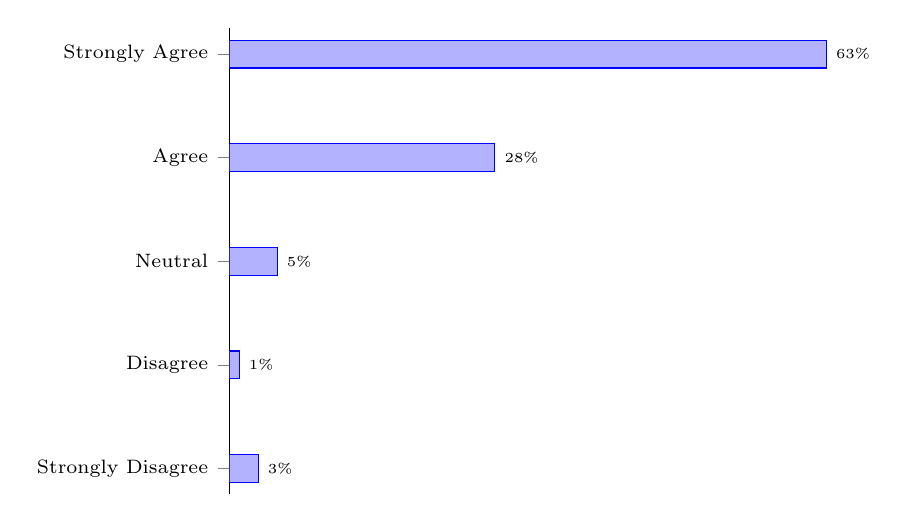
\begin{tikzpicture}
	\begin{axis}[
	axis x line=none,
	axis y line*=left,
	ytick={0,1,2,3,4},
	yticklabels={\scriptsize{Strongly Disagree}, \scriptsize{Disagree}, \scriptsize{Neutral}, \scriptsize{Agree}, \scriptsize{Strongly Agree}},
	xtick=\empty,
	xbar,
	xmin=0, xmax=70, ymin=-0.25, ymax=4.25,
	]
	
	\addplot coordinates {
		(3,0)
		(1,1)
		(5,2)
		(28,3)
		(63,4)
	};
	
	\draw (axis cs:3,0) |- (axis cs:3,0) node[near start,right]
	{\tiny{3\%}};
	\draw (axis cs:1,1) |- (axis cs:1,1) node[near start,right]
	{\tiny{1\%}};
	\draw (axis cs:5,2) |- (axis cs:5,2) node[near start,right]
	{\tiny{5\%}};
	\draw (axis cs:28,3) |- (axis cs:28,3) node[near start,right]
	{\tiny{28\%}};
	\draw (axis cs:63,4) |- (axis cs:63,4) node[near start,right]
	{\tiny{63\%}};
	\end{axis}
	\end{tikzpicture}
\end{center}
\end{frame}

\begin{frame}[fragile,t]
	\frametitle{One More Graph}
	
		\begin{center}
			\pgfplotsset{width=\textwidth,height=8.25cm,compat=1.3,tick label style={font=\tiny}}
			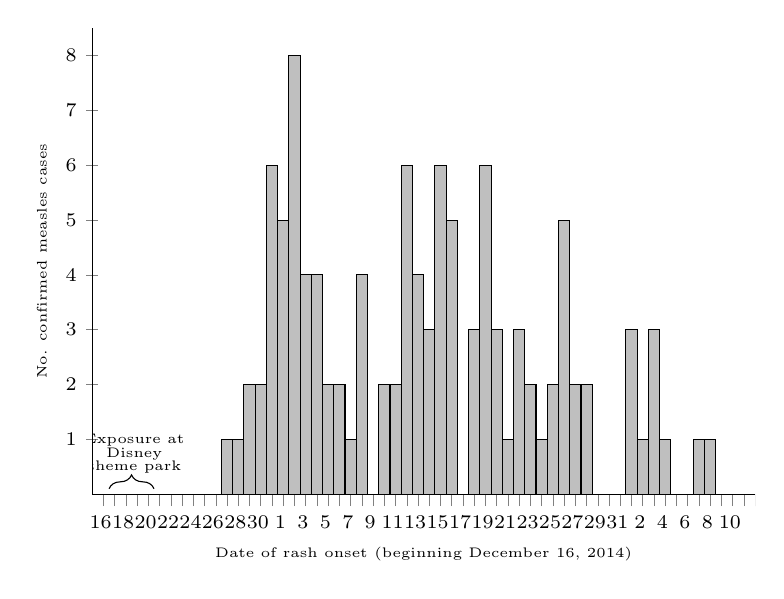
\begin{tikzpicture}
			\begin{axis}[
			axis x line=bottom,
			x axis line style=-,
			axis y line=left,
			y axis line style=-,
			ybar interval,
			xmajorgrids=false,
			ytick={1,2,3,4,5,6,7,8},
			yticklabels={1,2,3,4,5,6,7,8},
			ylabel style={font=\tiny},
			xtick={1,...,59},
			x tick label style={xshift=-.25cm},
			xlabel near ticks,
			xticklabels={,16,,18,,20,,22,,24,,26,,28,,30,,1,,3,,5,,7,,9,,11,,13,,15,,17,,19,,21,,23,,25,,27,,29,,31,,2,,4,,6,,8,,10,},
			xlabel style={font=\tiny},
			xlabel={Date of rash onset (beginning December 16, 2014)},
			ylabel={No. confirmed measles cases},
			ybar,
			xmin=0, xmax=59, ymin=0, ymax=8.5,
			]
			
			\addplot[const plot,fill=lightgray,draw=black] 
			coordinates{
				(11.5,0) (11.5,1) (12.5,0) (12.5,1) (13.5,0) (13.5,2) (14.5,0) (14.5,2) (15.5,0) (15.5,6) (16.5,0) (16.5,5) (17.5,0) (17.5,8) (18.5,0) (18.5,4) (19.5,0) (19.5,4) (20.5,0) (20.5,2) (21.5,0) (21.5,2) (22.5,0) (22.5,1) (23.5,0) (23.5,4) (24.5,0) (25.5,0) (25.5,2) (26.5,0) (26.5,2) (27.5,0) (27.5,6) (28.5,0) (28.5,4) (29.5,0) (29.5,3) (30.5,0) (30.5,6) (31.5,0) (31.5,5) 
				(32.5,0) (33.5,0) (33.5,3) (34.5,0) (34.5,6) (35.5,0) (35.5,3) (36.5,0) (36.5,1) (37.5,0) (37.5,3) (38.5,0) (38.5,2) (39.5,0) (39.5,1) (40.5,0) (40.5,2) (41.5,0) (41.5,5) (42.5,0) (42.5,2) (43.5,0) (43.5,2) (44.5,0) (45.5,0) (46.5,0) (47.5,0) (47.5,3) (48.5,0) (48.5,1) (49.5,0) (49.5,3) (50.5,0) (50.5,1) (51.5,0) (52.5,0) (53.5,0) (53.5,1) (54.5,0) (54.5,1) (55.5,0) (55.5,1) (55.5,0)
			}; closedcycle;
			
			\node at (axis cs:3.75,.7) [anchor=south,font=\tiny] {Exposure at};
			\node at (axis cs:3.75,.45) [anchor=south] {\tiny{Disney}};
			\node at (axis cs:3.75,.2) [anchor=south] {\tiny{theme park}};
			\draw [decorate, decoration={brace,amplitude=5pt}] (axis cs:1.5,.1)--(axis cs:5.5,.1) 
			node {};
			\node at (axis cs:8.5,0) [anchor=north,font=\tiny] {December};
			\addplot[smooth,domain=0:59]{0};
			\end{axis}
			\end{tikzpicture}
		\end{center}
\end{frame}

\begin{frame}[fragile,t]
\frametitle{Diagrams using tikz}

The tikz package is also great for generating diagrams of various types.

\bigskip

\begin{tcolorbox}[colback=red!5!white,colframe=red!75!black]
\begin{Verbatim}
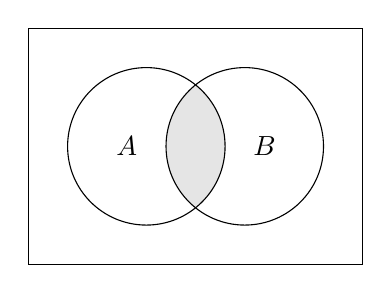
\begin{tikzpicture}
    \draw (-1.5,-1.5) rectangle (2.75,1.5);
    \begin{scope}
        \clip (0,0) circle (1);
        \fill[gray!20] (1.25,0) circle (1);
    \end{scope}
    \draw (0,0) circle (1);
    \draw (1.25,0) circle (1);
    \draw (-.25,0) node {$A$};
    \draw (1.5,0) node {$B$};
\end{tikzpicture}
\end{Verbatim}
\end{tcolorbox}
\end{frame}

\begin{frame}
	\frametitle{The Output}
\begin{center}
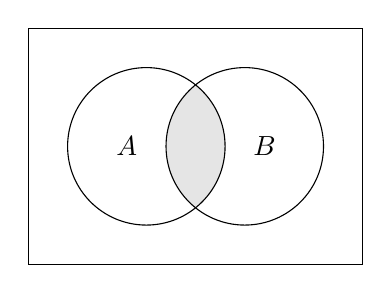
\begin{tikzpicture}
\draw (-1.5,-1.5) rectangle (2.75,1.5);
\begin{scope}
\clip (0,0) circle (1);
\fill[gray!20] (1.25,0) circle (1);
\end{scope}
\draw (0,0) circle (1);
\draw (1.25,0) circle (1);
\draw (-.25,0) node {$A$};
\draw (1.5,0) node {$B$};
\end{tikzpicture}
\end{center}	
\end{frame}

\begin{frame}[fragile]
\frametitle{A Circuit Diagram}

\begin{circuitikz}
	\draw
	% Drawing a npn transistor
	(0,0) node[npn](npn1){} 
	% Making connections from transistor using relative coordinates
	(npn1.E) node[right=7mm, above=5mm]{2N2222} % Labelling the transistor
	(npn1.B) -- ++(-1,0) to [R,l_=10<\kilo\ohm>,*-*] ++(0,-3)  
	(npn1.B) -- ++(-3,0) to [C,l_=100<\nano\farad>] ++(0,-3) node(gnd1){}
	(npn1.E) to [R,l_=10<\kilo\ohm>,*-*] (0,-3)
	(npn1.E) -- ++(2,0) to [C,l=10<\pico\farad>,*-*] (2,-3)
	(npn1.B) -- ++(-1,0) to [R,l_=10<\kilo\ohm>,*-] ++(0,3) node(con1){}
	(npn1.C) to [L,l_=150<\micro\henry>,*-] (0,3) 
	(npn1.C) -- ++(2,0) to [C,l=10<\pico\farad>,*-*] ++(0,-1.5)
	% Drawing shorts and ground connection
	(-1,3)to[short,*-o] (-1,4) node[right]{$V_{DD}=6 VDC$} % Power supply
	% Output sinusoidal waveform at approximately 50 MHz
	(npn1.C) -- ++(4,0) to [short,-o]
	++(0,0) node[right]{$V_o$}
	(0,-3) node[ground]{}% Define this node as ground
	(gnd1) ++(0,0) to[short,-o] ++(7.85,0)
	(con1)to[short] ++(1.85,0)
	;
\end{circuitikz}
\end{frame}

\begin{frame}[fragile]
\frametitle{The Chemical Structure of Caffine}

\begin{center}
\chemfig{*6((=O)-N(-CH_3)-*5(-N=-N(-CH_3)-=)--(=O)-N(-H_3C)-)}
\end{center}
\end{frame}

\begin{frame}[fragile]
	\frametitle{Commutative Diagrams}
	
	\begin{center}
	$$\begin{tikzcd}[row sep=scriptsize, column sep=scriptsize]
		& f^* E_V \arrow[dl] \arrow[rr] \arrow[dd] & & E_V \arrow[dl] \arrow[dd] \\ f^* E \arrow[rr, crossing over] \arrow[dd] & & E \\
		& U \arrow[dl] \arrow[rr] & & V \arrow[dl] \\
		M \arrow[rr] & & N \arrow[from=uu, crossing over]\\
	\end{tikzcd}$$
	\end{center}
\end{frame}

\begin{frame}
\frametitle{State Machines}

\begin{center}
		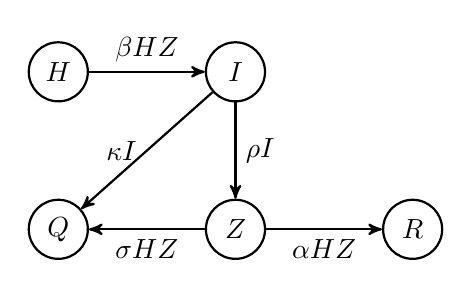
\begin{tikzpicture}[->,>=stealth']
		\node[state] (H) {$H$};
		\node[state, right of=H, node distance=2.25cm] (I) {$I$};
		\node[state, below of=H, node distance=2cm] (Q) {$Q$};
		\node[state, right of=Q, node distance=2.25cm] (Z) {$Z$};
		\node[state, right of=Z, node distance=2.25cm] (R) {$R$};
		
		\path
		(H) edge[thick] node[above]{$\beta H Z$} (I)
		(I) edge[thick] node[left]{$\kappa I$} (Q)
		(I) edge[thick] node[right]{$\rho I$} (Z)
		(Z) edge[thick] node[below]{$\sigma HZ$} (Q)
		(Z) edge[thick] node[below]{$\alpha HZ$} (R);
		\end{tikzpicture}
\end{center}
\end{frame}

\begin{frame}[t]
\frametitle{What To Do From Here}

\begin{enumerate}
\item Install \LaTeX\ on your computer.
\pause
\item Create the outline of your weekly update as a Beamer presentation.
\pause
\item Use the paper template provided to start using \LaTeX.  In this paper, pick a math ``problem" and recreate it.  Try and find something that uses interesting symbols and positionings so you can explore how to typeset mathematics.
\pause
\item Insert an image into the paper.  \pause (Keep it clean in the 2017)
\pause
\item Draw the graph of an interesting function or functions.
\pause
\item Plot data points of some sort.  This should be the recreation of a graph that has some meaning to you (perhaps from a paper that you have read to prepare for this REU?)
\pause
\item Explore what \LaTeX\ can do through google. 
\end{enumerate}
\end{frame}

\end{document}

\begin{frame}
	\frametitle{Commutative Diagrams}
	
	\begin{center}
		\begin{tikzcd}[row sep=scriptsize, column sep=scriptsize]
			& f^* E_V \arrow[dl] \arrow[rr] \arrow[dd] & & E_V \arrow[dl] \arrow[dd] \\ f^* E \arrow[rr, crossing over] \arrow[dd] & & E \\
			& U \arrow[dl] \arrow[rr] & & V \arrow[dl] \\
			M \arrow[rr] & & N \arrow[from=uu, crossing over]\\
		\end{tikzcd}
	\end{center}
\end{frame}

